% Figure 1 -- mechanism diagram for "Endogenous Credibility in Social Learning".
% Standalone TikZ; compile with: pdflatex fig1_mechanism.tex
\documentclass[border=5pt]{standalone}
\usepackage{amsmath,amssymb,bm}
\usepackage{tikz}
\usetikzlibrary{arrows.meta,positioning,fit,backgrounds,calc}

\begin{document}
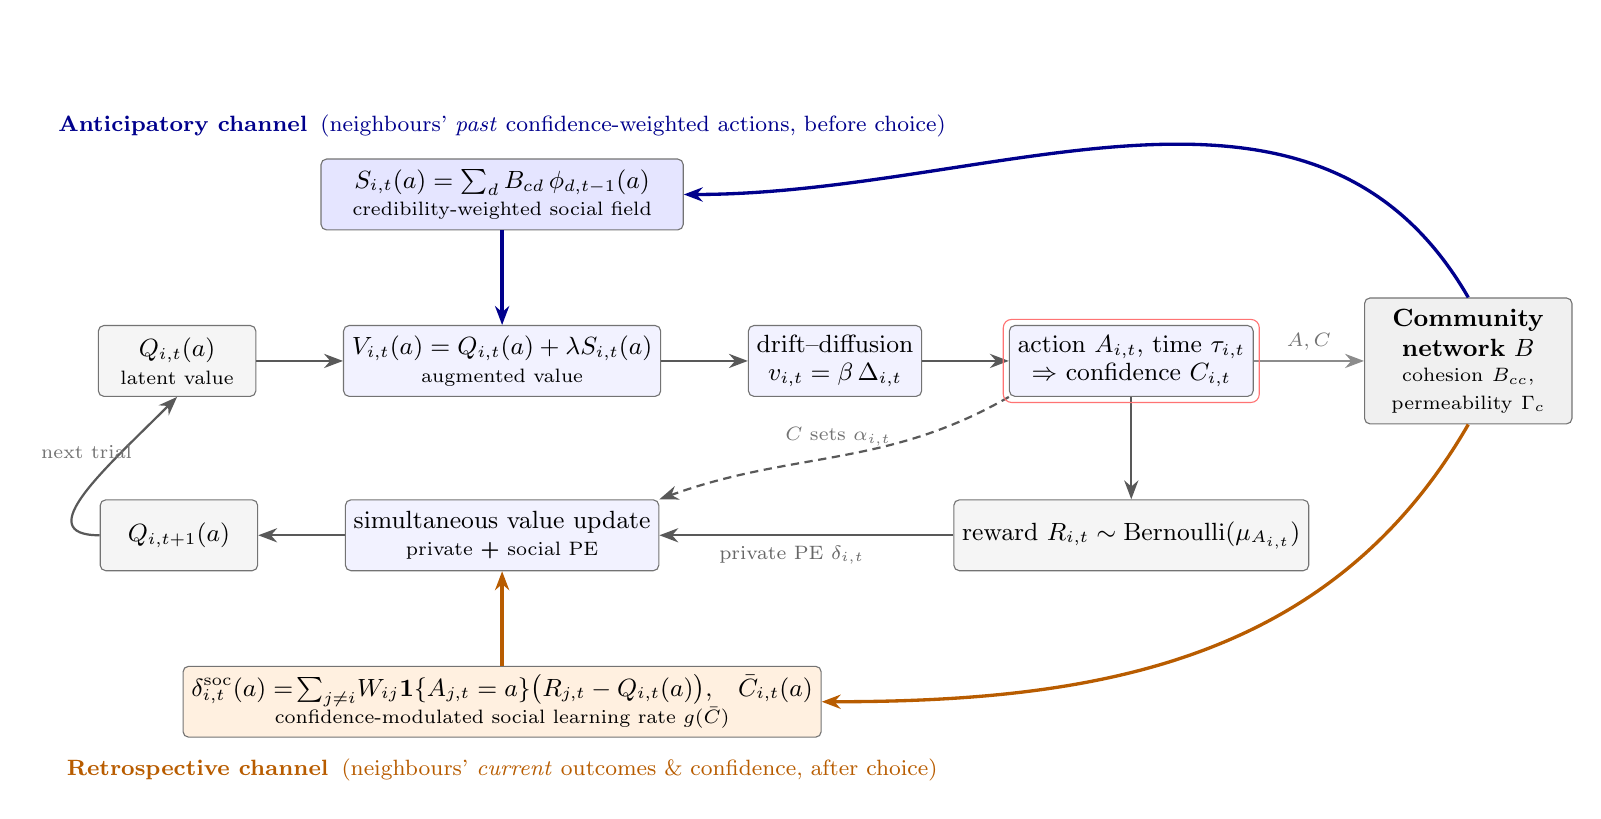
\begin{tikzpicture}[
  font=\small,
  >={Stealth[length=2.4mm]},
  box/.style={draw=black!55,rounded corners=2pt,align=center,
              minimum height=9mm,minimum width=20mm,inner sep=3pt},
  state/.style={box,fill=black!4},
  proc/.style={box,fill=blue!5},
  flow/.style={->,thick,black!65},
  ant/.style={->,very thick,blue!55!black},
  retro/.style={->,very thick,orange!72!black},
]

% ---- within-trial core pipeline (left to right) -------------------------
\node[state] (Q)   {$Q_{i,t}(a)$\\[-1pt]\scriptsize latent value};
\node[proc,right=11mm of Q]   (V)  {$V_{i,t}(a)=Q_{i,t}(a)+\lambda S_{i,t}(a)$\\[-1pt]\scriptsize augmented value};
\node[proc,right=11mm of V]   (DDM){drift--diffusion\\[-1pt]$v_{i,t}=\beta\,\Delta_{i,t}$};
\node[proc,right=11mm of DDM] (AC) {action $A_{i,t}$, time $\tau_{i,t}$\\[-1pt]$\Rightarrow$ confidence $C_{i,t}$};

\draw[flow] (Q)   -- (V);
\draw[flow] (V)   -- (DDM);
\draw[flow] (DDM) -- (AC);

% ---- environment + value update (lower row) -----------------------------
\node[state,below=13mm of AC]  (R)   {reward $R_{i,t}\sim\mathrm{Bernoulli}(\mu_{A_{i,t}})$};
\node[proc,below=13mm of V]    (upd) {simultaneous value update\\[-1pt]\scriptsize private \textbf{+} social PE};
\node[state,left=11mm of upd]  (Qn)  {$Q_{i,t+1}(a)$};

\draw[flow] (AC) -- (R);
\draw[flow] (R)  -- node[below,pos=0.55,black!60,font=\scriptsize]{private PE $\delta_{i,t}$} (upd);
\draw[flow] (upd) -- (Qn);
\draw[flow] (Qn.west) .. controls ($(Qn.west)+(-0.9,0)$) and ($(Q.south)+(-0.9,-0.9)$) .. (Q.south);
\node[black!55,font=\scriptsize] at ($(Q.south)+(-1.15,-0.7)$) {next trial};

% confidence regulates the private learning rate
\draw[flow,densely dashed] (AC.south west) to[out=210,in=20] node[above,pos=0.5,black!55,font=\scriptsize]{$C$ sets $\alpha_{i,t}$} (upd.north east);

% ---- anticipatory channel (top band) ------------------------------------
\node[box,fill=blue!10,above=12mm of V,minimum width=46mm] (S)
   {$S_{i,t}(a)=\sum_{d} B_{cd}\,\phi_{d,t-1}(a)$\\[-1pt]\scriptsize credibility-weighted social field};
\draw[ant] (S) -- (V);
\node[blue!55!black,font=\footnotesize,above=1.5mm of S]
   {\textbf{Anticipatory channel}\;\;(neighbours' \emph{past} confidence-weighted actions, before choice)};

% ---- retrospective channel (bottom band) --------------------------------
\node[box,fill=orange!12,below=12mm of upd,minimum width=58mm] (soc)
   {$\delta^{\mathrm{soc}}_{i,t}(a)=\!\sum_{j\neq i}\!W_{ij}\mathbf{1}\{A_{j,t}=a\}\bigl(R_{j,t}-Q_{i,t}(a)\bigr)$,\quad $\bar C_{i,t}(a)$\\[-1pt]\scriptsize confidence-modulated social learning rate $g(\bar C)$};
\draw[retro] (soc) -- (upd);
\node[orange!72!black,font=\footnotesize,below=1.5mm of soc]
   {\textbf{Retrospective channel}\;\;(neighbours' \emph{current} outcomes \& confidence, after choice)};

% ---- community coupling (right) -----------------------------------------
\node[draw=black!55,rounded corners=2pt,fill=black!6,align=center,
      right=14mm of AC,minimum height=16mm,text width=24mm] (net)
   {\textbf{Community}\\\textbf{network} $B$\\[1pt]\scriptsize cohesion $B_{cc}$,\\[-1pt]\scriptsize permeability $\Gamma_c$};
\draw[ant]   (net.north) to[out=120,in=0] (S.east);
\draw[retro] (net.south) to[out=240,in=0] (soc.east);
\draw[flow,black!45] (AC.east) -- node[above,font=\scriptsize,black!55]{$A,C$} (net.west);

% ---- highlight that confidence is the shared link ----------------------
\node[draw=red!55,rounded corners=3pt,inner sep=2pt,fit=(AC)] {};

\end{tikzpicture}
\end{document}
